% ============================================================
\section{Development}
\label{sec:development}

This chapter describes the implementation of the visionOS frontend and Python backend pipeline shown in Figure~\ref{fig:sysdesign}. Under ADP constraints, the headset provides interaction and tracking signals, while RGB is acquired via AirPlay mirroring (UxPlay) and depth is provided by an external RealSense sensor.

\subsection{Development Setup}
\label{subsec:dev_setup}

\subsubsection{Hardware and Deployment Layout}

Development used a Mac mini for visionOS development and UxPlay mirroring during integration, an Apple Vision Pro headset for device testing, and a Linux GPU server for running the backend services and pose inference. An Intel RealSense camera provides metric RGB-D input.

\begin{table}[H]
    \centering
    \caption{Hardware overview}
    \label{tab:hw_overview_impl}
    \begin{tabular}{p{0.30\linewidth}p{0.58\linewidth}}
        \toprule
        \textbf{Component} & \textbf{Notes} \\
        \midrule
        Mac mini (M2) & Xcode/visionOS development; optional UxPlay receiver host. \\
        Apple Vision Pro & On-device testing for UI, tracking, immersive rendering. \\
        Linux GPU server & Runs Python CV service and Dockerized pose inference. \\
        Intel RealSense & External RGB-D sensing; aligned depth-to-color via SDK. \\
        \bottomrule
    \end{tabular}
\end{table}
\subsubsection{Software Stack}
The implementation is organized into four software components: the visionOS client, a Python computer-vision backend, a separate GPU-backed pose inference service, and a small set of calibration utilities. The visionOS application is implemented in Swift and uses SwiftUI for windowed UI, ARKit for device/world tracking, and RealityKit for immersive 3D rendering and pose overlays. The main CV backend is implemented in Python and exposed through a \texttt{Flask} service running in a \texttt{uv} environment; it ingests the mirrored RGB stream from UxPlay, acquires and aligns RealSense RGB-D, loads calibration parameters, performs camera-to-camera registration and depth reprojection, synthesizes ROI masks, exposes debug visualizations, and orchestrates requests to the pose estimator. Pose inference is executed by a separate Dockerized REST service integrating FoundationPose on the GPU server. Finally, calibration scripts based on OpenCV are used to estimate intrinsics/distortion parameters and to support ArUco-based pose estimation for registration.

\begin{table}[H]
    \centering
    \caption[Software stack overview]{Software stack overview.}
    \label{tab:sw_stack_impl}
    \begin{tabular}{p{0.30\linewidth}p{0.58\linewidth}}
        \toprule
        \textbf{Component} & \textbf{Role} \\
        \midrule
        visionOS app (Swift) & SwiftUI UI windows; ARKit tracking; RealityKit overlays. \\
        CV backend (Python) & \texttt{Flask} service: UxPlay ingestion, RealSense capture/alignment, calibration loading, registration, depth reprojection, ROI masks, debug endpoints, orchestration. \\
        Pose inference service & Dockerized REST service running FoundationPose on the GPU server. \\
        Calibration utilities & OpenCV scripts for intrinsics/distortion estimation and ArUco detection. \\
        \bottomrule
    \end{tabular}
\end{table}

\subsubsection{Auxiliary Modules Used During Development}
Two auxiliary tools were used during implementation and debugging to decouple failure analysis from the full AVP--backend integration. A lightweight Streamlit frontend, developed by a colleague, was used to submit pose jobs (RGB, depth, mask, mesh) directly to the pose inference API and visualize the outputs, providing a fast way to validate inference behavior independently of the visionOS client and the reprojection pipeline. In addition, a minimal ``quick-test'' Python script provided by the supervisor enabled deterministic replay of saved request folders, supporting rapid regression testing and repeatable reproduction of inference failures.

\begin{table}[H]
    \centering
    \caption[Auxiliary development tools]{Auxiliary tools used for debugging and regression testing.}
    \label{tab:aux_tools_impl}
    \begin{tabular}{p{0.30\linewidth}p{0.58\linewidth}}
        \toprule
        \textbf{Tool} & \textbf{Use during implementation} \\
        \midrule
        Streamlit frontend (colleague) & Direct submission of (RGB, depth, mask, mesh) to the pose API with result visualization, independent of AVP and reprojection. \\
        Quick-test replay script (supervisor) & Deterministic replay of saved request folders for regression testing and reproduction of inference failures. \\
        \bottomrule
    \end{tabular}
\end{table}


\subsubsection{Mixed-Reality Development Workflow}

Mac Virtual Display was used to work on the Mac mini from within AVP. Figure~\ref{fig:mac_virtual_display} is a placeholder illustration. While it offers an futuristic and relaxing development environment, it can induce an ``infinite mirror'' effect when mirrored debug windows are visible and can be visually tiring during long debugging sessions.

\begin{figure}[H]
\centering
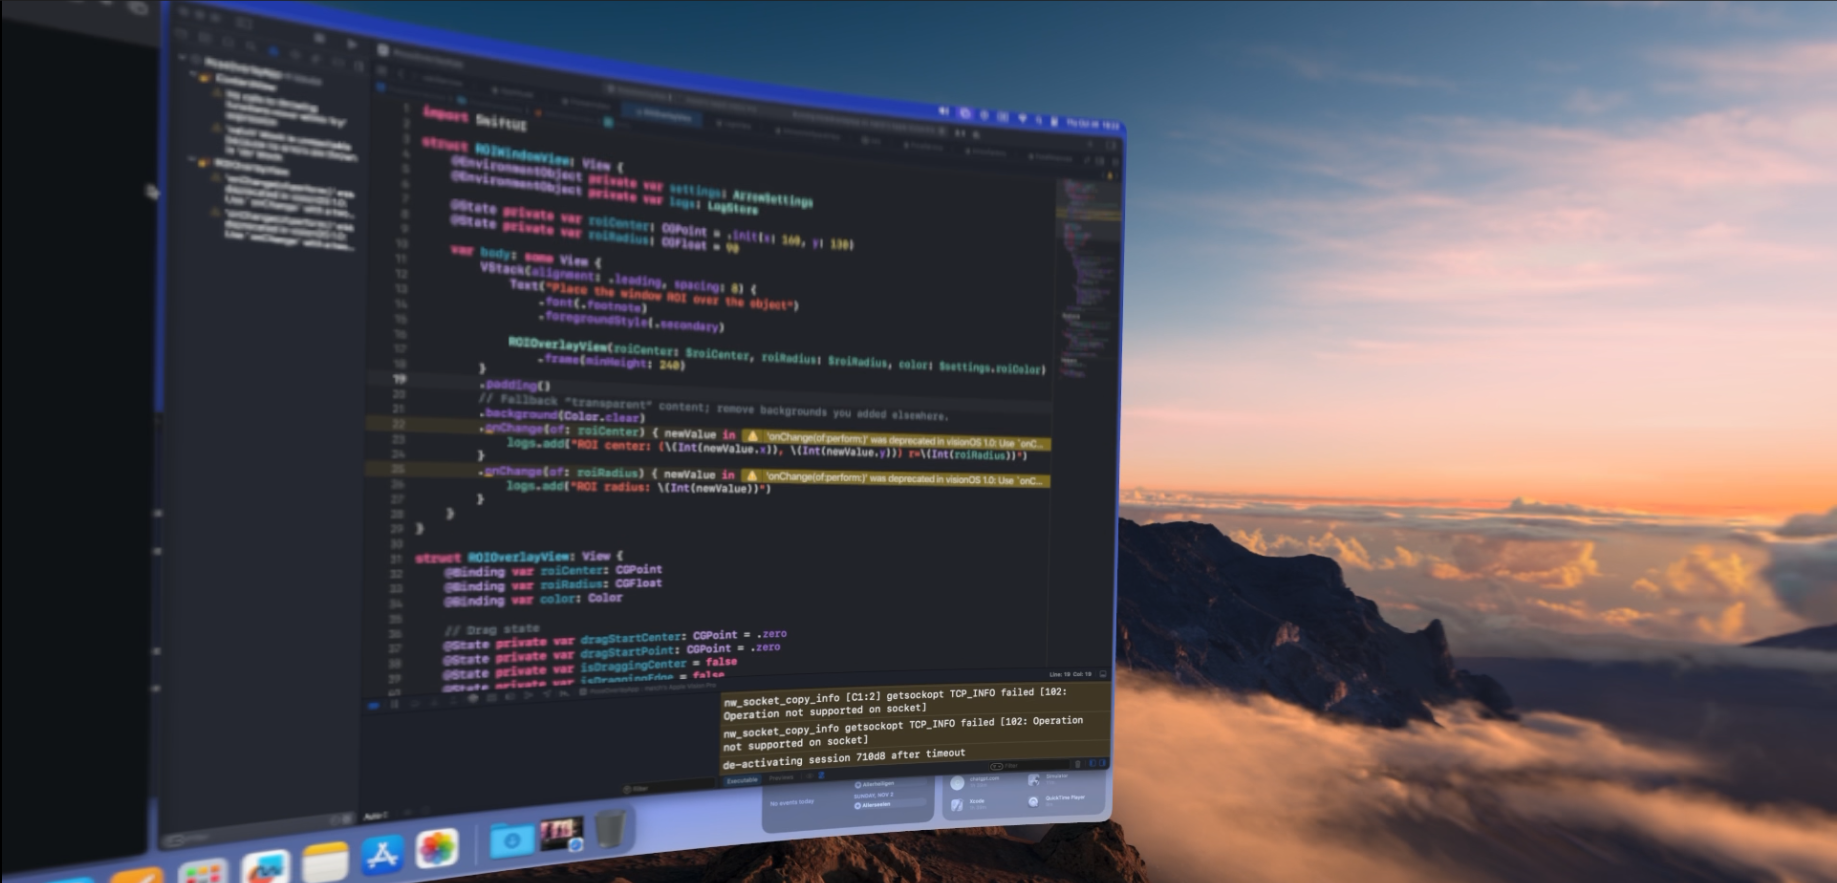
\includegraphics[width=\textwidth]{figures/ardevenv.png}
\caption{Illustration of the Mac Virtual Display workflow used during development.}
\label{fig:mac_virtual_display}
\end{figure}
\subsubsection{Xcode and visionOS Workflow}
\label{subsec:xcode_workflow}

The visionOS project was implemented as a thin controller and visualization layer. For repeatable builds and reliable device testing, several Xcode and runtime practices proved important. Development primarily used the \texttt{Debug} configuration for rapid iteration (e.g., verbose logging and fast incremental builds), while \texttt{Release} builds were used for performance checks. Build and run configurations are managed per scheme in Xcode via \emph{Product} $\rightarrow$ \emph{Scheme} $\rightarrow$ \emph{Edit Scheme}, where build, run, test, and archive settings can be configured independently.

On-device deployment further requires correct signing and provisioning. A valid development team selection and a matching provisioning profile must be configured; misconfiguration typically manifests as install or deployment failures rather than compile-time errors. With respect to permissions, the application avoids camera entitlements because raw camera access is not available under ADP. Instead, it relies on ARKit tracking and network communication, and the \texttt{Info.plist} includes the required usage descriptions for local network access and motion/world tracking to enable these capabilities.

To reduce rebuilds during integration, runtime parameters such as backend host/port and model selection are configurable within the application. For debugging, key state variables (e.g., ROI parameters, active mesh, latest pose, and connection status) are exposed through dedicated UI windows, which minimizes reliance on external debug pages during iterative testing.


\subsubsection{Pose Inference Backend (REST API)}
\label{subsec:pose_api}

Pose inference is performed by a Dockerized REST service running on the GPU server. It processes one object per request (one mesh + one mask, optionally across multiple frames), returns one $\mathrm{SE}(3)$ matrix per frame, and stores each job to disk for reproducibility and offline replay. The model is loaded once at server startup and requests are processed sequentially.

\begin{table}[H]
\centering
\caption{Pose API request/response scheme (base64-encoded binary inside JSON).}
\label{tab:pose_api_io}
\begin{tabular}{p{0.34\linewidth}p{0.58\linewidth}}
\toprule
\textbf{Field} & \textbf{Description} \\
\midrule
\texttt{POST /foundationpose} & Inference endpoint for a single job. \\
\texttt{camera\_matrix} & $3\times 3$ intrinsics $\mathbf{K}$ (row-major JSON array). \\
\texttt{images[i].rgb} & Base64 PNG (RGB frame $i$). \\
\texttt{images[i].depth} & Base64 PNG (depth frame $i$, aligned to RGB). \\
\texttt{mask} & Base64 PNG (binary mask; applies to all frames). \\
\texttt{mesh} & Base64 PLY (mesh; applies to all frames). \\
\texttt{transformation\_matrix[i]} & $4\times 4$ $\mathbf{T}_{C \leftarrow O}$ for frame $i$ (row-major). \\
\bottomrule
\end{tabular}
\end{table}
\subsection{System Modules}

\subsubsection{Camera Intrinsics and Distortion}
\label{subsec:impl_calibration}
Accurate intrinsics and distortion parameters are required for depth back-projection, cross-camera reprojection, and consistent overlay rendering. For the UxPlay (mirrored AVP) view, these parameters are not accessible under ADP and are therefore estimated offline using an explicit calibration procedure. The resulting pinhole intrinsics and Brown--Conrady distortion coefficients are stored as JSON and loaded by the backend at startup,
\[
\mathbf{K}_{AVP}, \quad \mathbf{d}_{AVP} = [k_1,k_2,p_1,p_2,k_3].
\]
For the RealSense color stream, intrinsics and distortion are obtained directly from the RealSense SDK, and depth is aligned to the color frame using the SDK alignment primitive to ensure consistent geometry for subsequent back-projection. RealSense alignment and intrinsics extraction are illustrated in Listing~\ref{lst:rs_align_backproject}. The distortion model and calibration objective are detailed in Appendix~\ref{app:math_full}.

\subsubsection{RGB-D Alignment and Depth Reprojection}
\label{subsec:impl_reprojection}
Aligned RealSense depth is transformed into the UxPlay view using a camera-to-camera registration derived from paired ArUco detections. Given marker poses estimated independently in the RealSense and UxPlay camera frames, the transform is computed as
\[
\mathbf{T}_{AVP \leftarrow RS} =
\mathbf{T}_{AVP \leftarrow M}\left(\mathbf{T}_{RS \leftarrow M}\right)^{-1},
\]
as implemented in Listing~\ref{lst:aruco_Tavprs}. Depth reprojection then follows the standard sequence of back-projecting aligned depth pixels into 3D, transforming points into the UxPlay camera frame, and projecting them into the UxPlay image plane while applying distortion and resolving collisions via z-buffering. A representative implementation excerpt is provided in Listing~\ref{lst:depth_to_avp}, while the complete derivation and collision handling are documented in Appendix~\ref{app:math_full}, Section~\ref{app:depth_reprojection_full}.

\subsubsection{ROI Masks and Interaction}
\label{subsec:impl_roi}
The final system represents the ROI by normalized parameters $(c_x,c_y,r)$ provided by the visionOS client. The backend converts these parameters into an analytic circular mask in UxPlay image coordinates, avoiding color-based reconstruction and contour extraction. The corresponding implementation is shown in Listing~\ref{lst:avp_roi_mask}. Earlier ROI concepts relied on HSV thresholding of colored overlays (ring or freeform contours) rendered into the mirrored stream; active-contour refinement was considered as a potential post-processing step but was not adopted due to tuning sensitivity and additional runtime cost.

\subsubsection{Debugging Views and System Introspection}
\label{subsec:impl_debug}
To support systematic debugging, the backend exposes endpoint-based visualizations for intermediate outputs, including mirrored RGB frames, RealSense RGB/depth, ROI masks, reprojected depth in UxPlay coordinates, and pose overlays. Figure~\ref{fig:debug_dashboard_placeholder} shows the debug endpoint used to inspect the pipeline stages during integration. A complete list of endpoints and their usage is provided in Appendix~\ref{app:system_usage}.

\begin{figure}[H]
\centering
\fbox{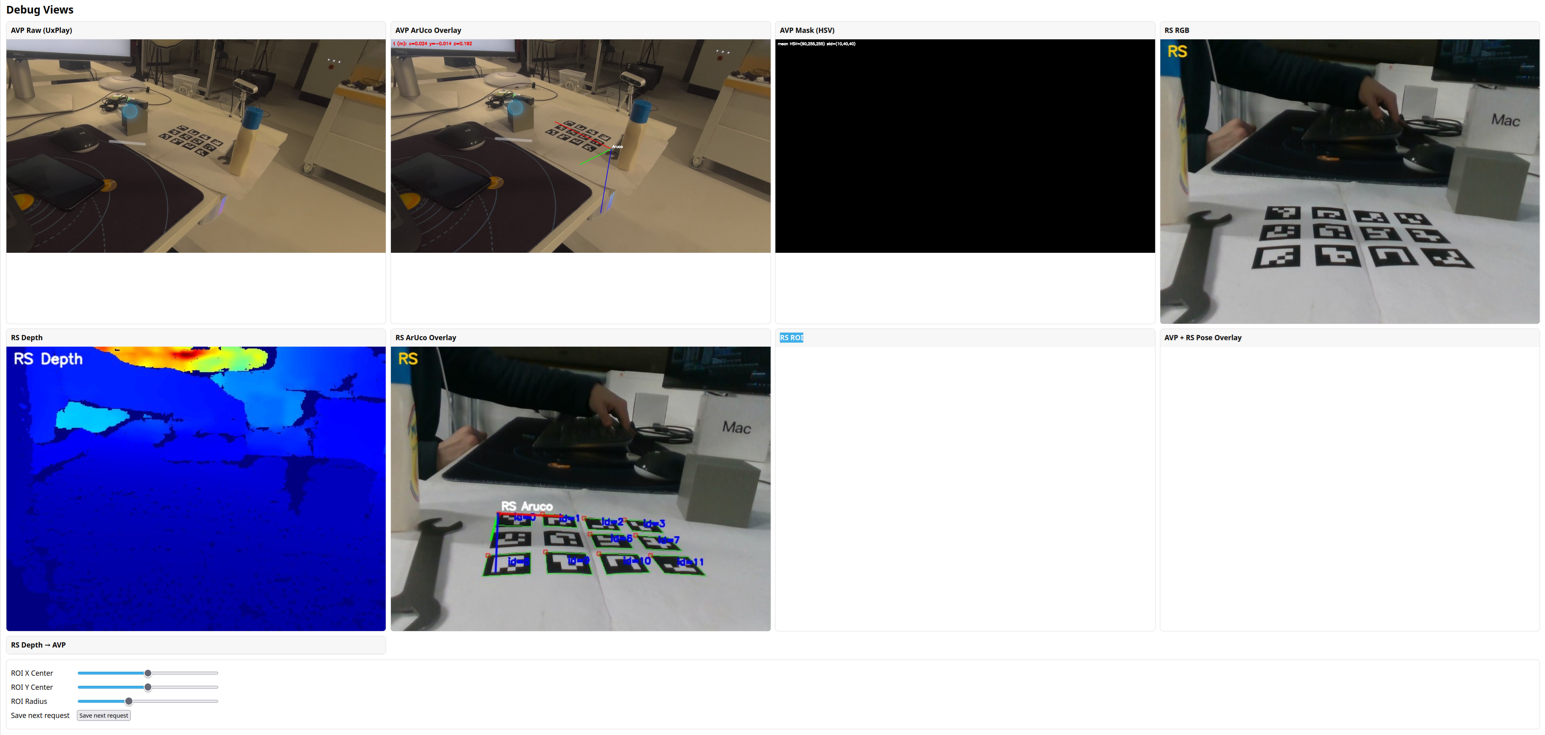
\includegraphics[width=0.95\textwidth]{figures/debugging_endpoint.png}}
\caption[Debug endpoint]{Debug endpoint used to inspect intermediate pipeline outputs.}
\label{fig:debug_dashboard_placeholder}
\end{figure}

\subsubsection{Pose Inference and Payload Assembly}
\label{subsec:impl_pose_payload}
Pose estimation is executed by a separate REST service, and the CV backend acts as an orchestrator that assembles and submits inference requests. Payload construction includes camera intrinsics, RGB and depth images, the ROI mask, and the selected mesh model, encoded for transport. A representative excerpt of the payload assembly is shown in Listing~\ref{lst:pose_api_payload}.

\subsubsection{Pose Visualization Outputs}
\label{subsec:impl_visualization}
Pose results are visualized in two complementary ways. First, 2D overlays are rendered in the UxPlay image plane (e.g., projected axes and mesh cues) to enable direct verification of camera-frame consistency. Second, immersive 3D overlays can render world axes, marker axes, the RealSense camera pose, and the estimated object pose in AVP space once world registration is available. World-space overlays depend on device/world tracking together with a calibrated device-to-camera offset, and continuous marker tracking under brief occlusions is handled by caching $\mathbf{T}_{D \leftarrow M}$ at detection time, as described in Appendix~\ref{app:math_full}, Section~\ref{app:device_anchor_tracking_full}.
